% Asset ID: FA22GameTheoryEnrichmentTikZ-003
% Source: Transcript linear programming section
% Core CCEA status: Optional enrichment only
\documentclass[tikz,border=8pt]{standalone}
\usepackage{amsmath}
\usetikzlibrary{arrows.meta,positioning}
\definecolor{Canvas}{HTML}{FAF9F6}\definecolor{Ivory}{HTML}{FFFFF0}\definecolor{LineGrey}{HTML}{E5E5EA}\definecolor{AccentGold}{HTML}{C5A059}\definecolor{DeepGold}{HTML}{D4AF37}\definecolor{SoftPink}{HTML}{FBEFEF}\definecolor{MathText}{HTML}{2C2C2E}
\begin{document}
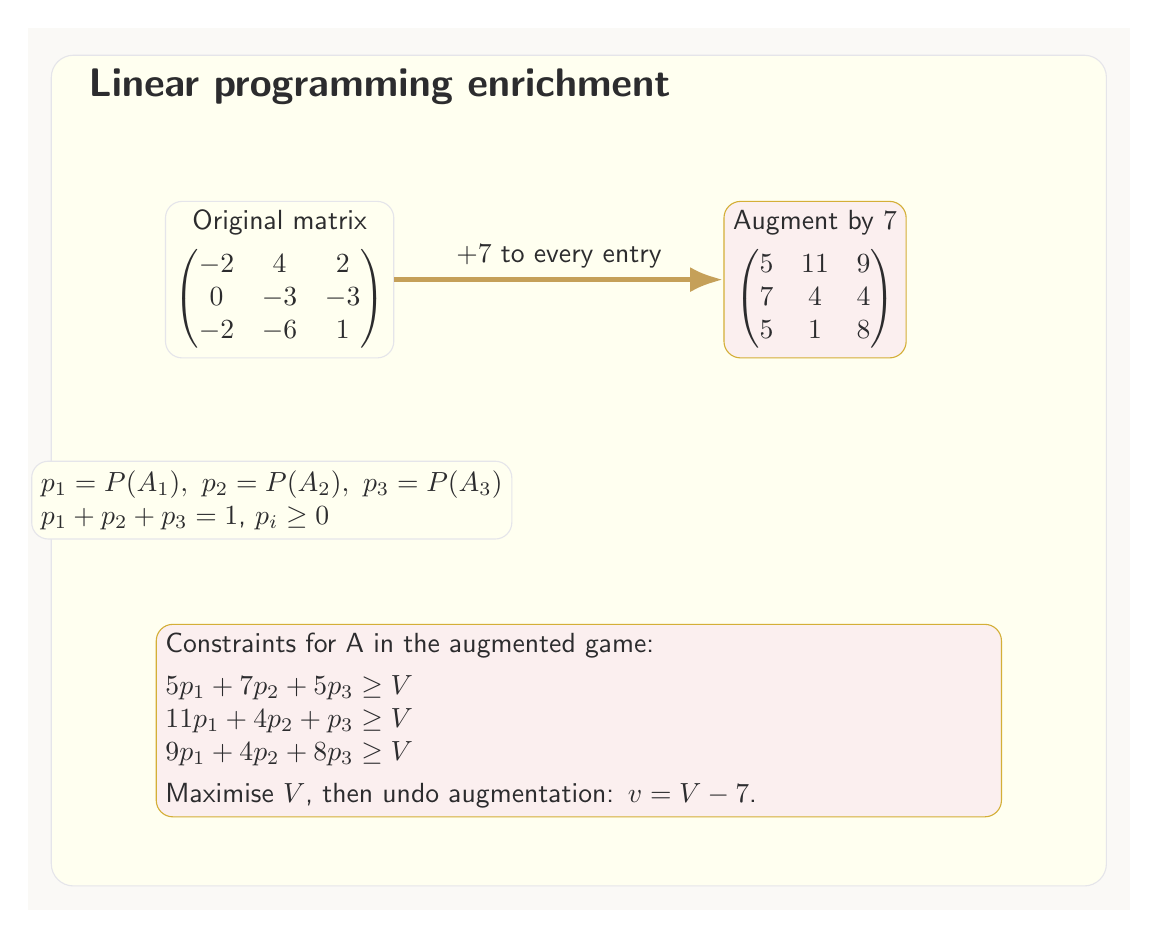
\begin{tikzpicture}[>=Latex,every node/.style={font=\sffamily,text=MathText}]
\fill[Canvas] (-7,-5.8) rectangle (7,5.4); \draw[LineGrey,fill=Ivory,rounded corners=8pt] (-6.7,-5.5) rectangle (6.7,5.05);
\node[anchor=west,font=\sffamily\bfseries\Large] at (-6.35,4.65){Linear programming enrichment};
\node[draw=LineGrey,fill=Ivory,rounded corners=6pt,align=center] (a) at (-3.8,2.2){Original matrix\\[4pt]\(\begin{pmatrix}-2&4&2\\0&-3&-3\\-2&-6&1\end{pmatrix}\)};
\node[draw=DeepGold,fill=SoftPink,rounded corners=6pt,align=center] (b) at (3,2.2){Augment by \(7\)\\[4pt]\(\begin{pmatrix}5&11&9\\7&4&4\\5&1&8\end{pmatrix}\)};
\draw[AccentGold,line width=2pt,-Latex] (a)--node[above]{\(+7\) to every entry}(b);
\node[draw=LineGrey,fill=Ivory,rounded corners=6pt,align=left] at (-3.9,-.6){\(p_1=P(A_1),\ p_2=P(A_2),\ p_3=P(A_3)\)\\\(p_1+p_2+p_3=1\), \(p_i\ge0\)};
\node[draw=DeepGold,fill=SoftPink,rounded corners=6pt,align=left,text width=10.5cm] at (0,-3.4){Constraints for A in the augmented game:\\[3pt]\(5p_1+7p_2+5p_3\ge V\)\\\(11p_1+4p_2+p_3\ge V\)\\\(9p_1+4p_2+8p_3\ge V\)\\[3pt]Maximise \(V\), then undo augmentation: \(v=V-7\).};
\end{tikzpicture}
\end{document}
